\documentclass{article}%
\usepackage[T1]{fontenc}%
\usepackage[utf8]{inputenc}%
\usepackage{lmodern}%
\usepackage{textcomp}%
\usepackage{lastpage}%
\usepackage[head=40pt,margin=0.5in,bottom=0.6in]{geometry}%
\usepackage{graphicx}%
%
\title{\textbf{Jubilados de Pdvsa protestaron por incumplimiento de pago en dólares}}%
\author{EL NACIONAL WEB}%
\date{08/10/2018}%
%
\begin{document}%
\normalsize%
\maketitle%
\textbf{URL: }%
http://www.el{-}nacional.com/noticias/protestas/jubilados{-}pdvsa{-}protestaron{-}por{-}incumplimiento{-}pago{-}dolares\_254856\newline%
%
\textbf{Periodico: }%
EN, %
ID: %
254856, %
Seccion: %
Protestas\newline%
%
\textbf{Palabras Claves: }%
Protestas\newline%
%
\textbf{Derecho: }%
2.6, %
Otros Derechos: %
2.3, %
Sub Derechos: %
2.6.1, 2.3.4\newline%
%
\textbf{EP: }%
SI\newline%
\newline%
%
\textbf{\textit{Las personas aseguraron que la compañía sacó bonos petroleros del fondo de pensionados~}}%
\newline%
\newline%
%
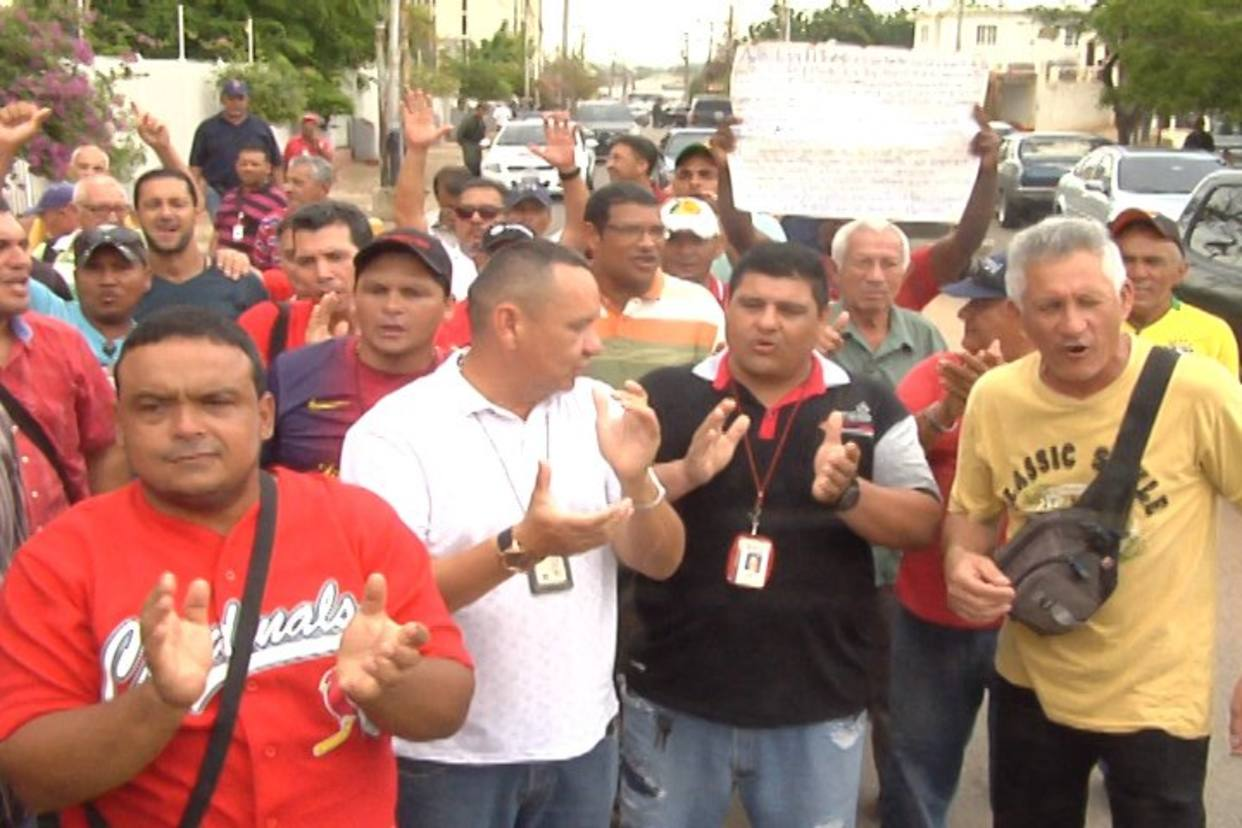
\includegraphics[width=300px]{247.jpg}%
\newline%
%
Un grupo de jubilados de Petróleos de Venezuela (Pdvsa) protestó este lunes por el incumplimiento de una deuda en dólares por parte de la estatal petrolera.%
\newline%
%
La actividad se llevó a cabo en las afueras del edificio Miranda, en Maracaibo.%
\newline%
%
Douglas Pereira, representante de los jubilados, explicó que las personas reclaman 2.600 millones de dólares;~producto de los bonos petroleros que Pdvsa sacó del fondo de pensionados en 2014.%
\newline%
%
“Deben distribuir~ 600 dólares mensuales en el lapso de un años por cada jubilado.Nos deben unos excedentes de 2016 para llegar a una pensión de entre 5.000 y hasta 6.000 bolívares soberanos”, dijo.%
\newline%
%
Aseguró que lograron reunirse con el personal administrativo de la compañía. “Ya logramos con esta protesta que se instalara una mesa para las 2:00 pm con las autoridades nacionales de Petróleos de Venezuela y los administradores”, agregó.%
\newline%
%
\end{document}